\documentclass{article}
\usepackage{graphicx}
\usepackage{geometry}
\usepackage{hyperref}
\usepackage{minted}
\usepackage{booktabs}
\usepackage{tabularx}
\usepackage{babel}
\usepackage{multirow}
\usepackage[autostyle]{csquotes}
\usepackage[T1]{fontenc}
\usepackage{parskip}
\usepackage{array}
\selectlanguage{ngerman}
\geometry{a4paper, margin=1in}



\title{Grundlagen von Datenbanksystemen - Projekt exist-Gründungsförderung}

\author{Jasper Liang, Frederik Gräven}
\date{Mai 2026}

\begin{document}
\maketitle
\newpage
\tableofcontents
\newpage
\section{Anforderungsanalyse}
\subsection{Einleitung}
exist ist ein Förderprogramm des Bundesministeriums für Wirtschaft und Energie. Ziel des Förderprogramms ist es die Anzahl der Unternehmensgründungen im Hochschul- und Forschungskontext zu erhöhen. Personen welche an einer Unternehmensgründung interessiert sind werden sowohl finanziell als auch informell unterstützt. Zu den möglichen Förderprogrammen zählen das exist Gründungsstipendium, exist Women und exist Forschungstransfer. \\
\textbf{exist-Gründungsstipendium} \\
Das exist Gründungsstipendium richtet sich an Studierende, Absolvierende und Wissenschaftler:innen aus Hochschulen und außeruniversitären Forschungseinrichtungen mit einer innovativen, technologieorientierten oder wissenbasierten Produktidee sowie signifikanten Alleinstellungsmerkmalen und guten wirtschaftlichen Erfolgsaussichten.\\
\textbf{exist-Women}\\
exist Women richtet sich speziell an Frauen und soll bei der Ideenfindung und Weiterentwicklung von Gründungsideen, sowie der Vernetzung und der Bildung eines Gründungsteams helfen. \\
\textbf{exist-Forschungstransfer}\\
exist Forschungstransfer soll potentielle Gründer:innen aus der Forschung bei der Unternehmensgründung unterstützen. Es besteht aus zwei Förderphasen. In Förderphase 1 sollen die Geschäftsideen zu einem Businessplan ausgearbeitet werden und Fragen im Zusammenhang mit der Umsetzung geklärt werden.
In Förderphase 2 geht es um die Finanzierung und Aufnahme der Geschäftstätigkeit

\subsection{Systembeschreibung}
Das System dient zur Einreichung, Verwaltung und Überprüfung von Anträgen der Förderprogramme exist-Gründungsstipendium, exist-Women und exist-Forschungstransfer. Forschungseinrichtungen sollen Anträge für Gründerteams einreichen und deren Status einsehen können. Bearbeiter:innen sollen den Antrag überprüfen und ablehnen/bewilligen sowie eine Notiz hinterlassen können.

\subsection{Vergleich Förderprogramme}
\begin{table}[htbp]
\centering

\begin{tabularx}{\textwidth}{l>{\raggedright\arraybackslash}p{3.5cm}>{\raggedright\arraybackslash}X}
\toprule
Name & Zielgruppe & Ziel & \\
\midrule
exist-Gründungsstipendium & Absolvent:innen oder Studierende & Entwicklung einer Geschäftsidee und vorbereitung Unternehmensgründung\\
exist-Women & Frauen & Vernetzung und Aufbau Gründungsteam, Ideenentwicklung\\
exist-Forschungstransfer & Forscher:innen & Überführung von Forschungsergebnisse in marktfähige Proukte und Aufbau eines Unternehmens\\
\bottomrule
\end{tabularx}
\caption{Vergleich Förderprogramme}
\end{table}

\newpage

\subsection{Systemgrenzen}
\textbf{Das System soll:}
\begin{itemize}
    \item Benutzer verwalten
    \item unterschiedliche Förderanträge speichern und verwalten
    \item Status eines Förderantrags anzeigen und verändern
    \item Notizen zu einem Förderantrag hinzufügen 
    \item Daten eines Förderantrags anzeigen
\end{itemize}
\newline
\textbf{Das System soll nicht:} 
\begin{itemize}
    \item Fördermittelauszahlung verwalten
    \item E-Mail Verkehr verwalten
    \item rechtliche Elemente verwalten
    \item vertragliche Elemente verwalten
    \item direkte Kommunikation ermöglichen
\end{itemize}
\subsection{Benutzer}

\begin{table}[htbp]
\centering
\begin{tabularx}{\textwidth}{lX}
\midrule
Gründerteam & Team welches sich mit einer Geschäftsidee für die Gründungsförderung bewirbt und ein Unternehmen Gründen möchte\\
Forschungseinrichtung & Antragstellende Einrichtung, welche das Gründungsteam unterstützt\\
Bearbeiter:in (PTJ-Projektträger Jülich) & Person, welche den Förderantrag überprüft und über Ablehnung oder Annahme entscheidet\\
\bottomrule
\end{tabularx}
\caption{Benutzer}
\end{table}

\subsection{Förderprozess}
\begin{itemize}
    \item[1] Forschungeseinrichtung füllt Förderantrag aus 
    \item[2] Förderantrag wird gespeichert und Forschungseinrichtung darüber informiert
    \item[3] Förderantrag erhält Status eingereicht
    \item[4] Bearbeiter:in prüft den Förderantrag
    \item[5] Bei Rückfragen wird Notiz angelegt
    \item[6] Förderantrag wird genehmigt oder abgelehnt
    \item[7] Status wird aktualisert
    \item[8] Gründungsteam und Forschungseinrichtung können Förderungsantrag einsehen
\end{itemize}

\subsection{Use Cases}

\begin{center}
    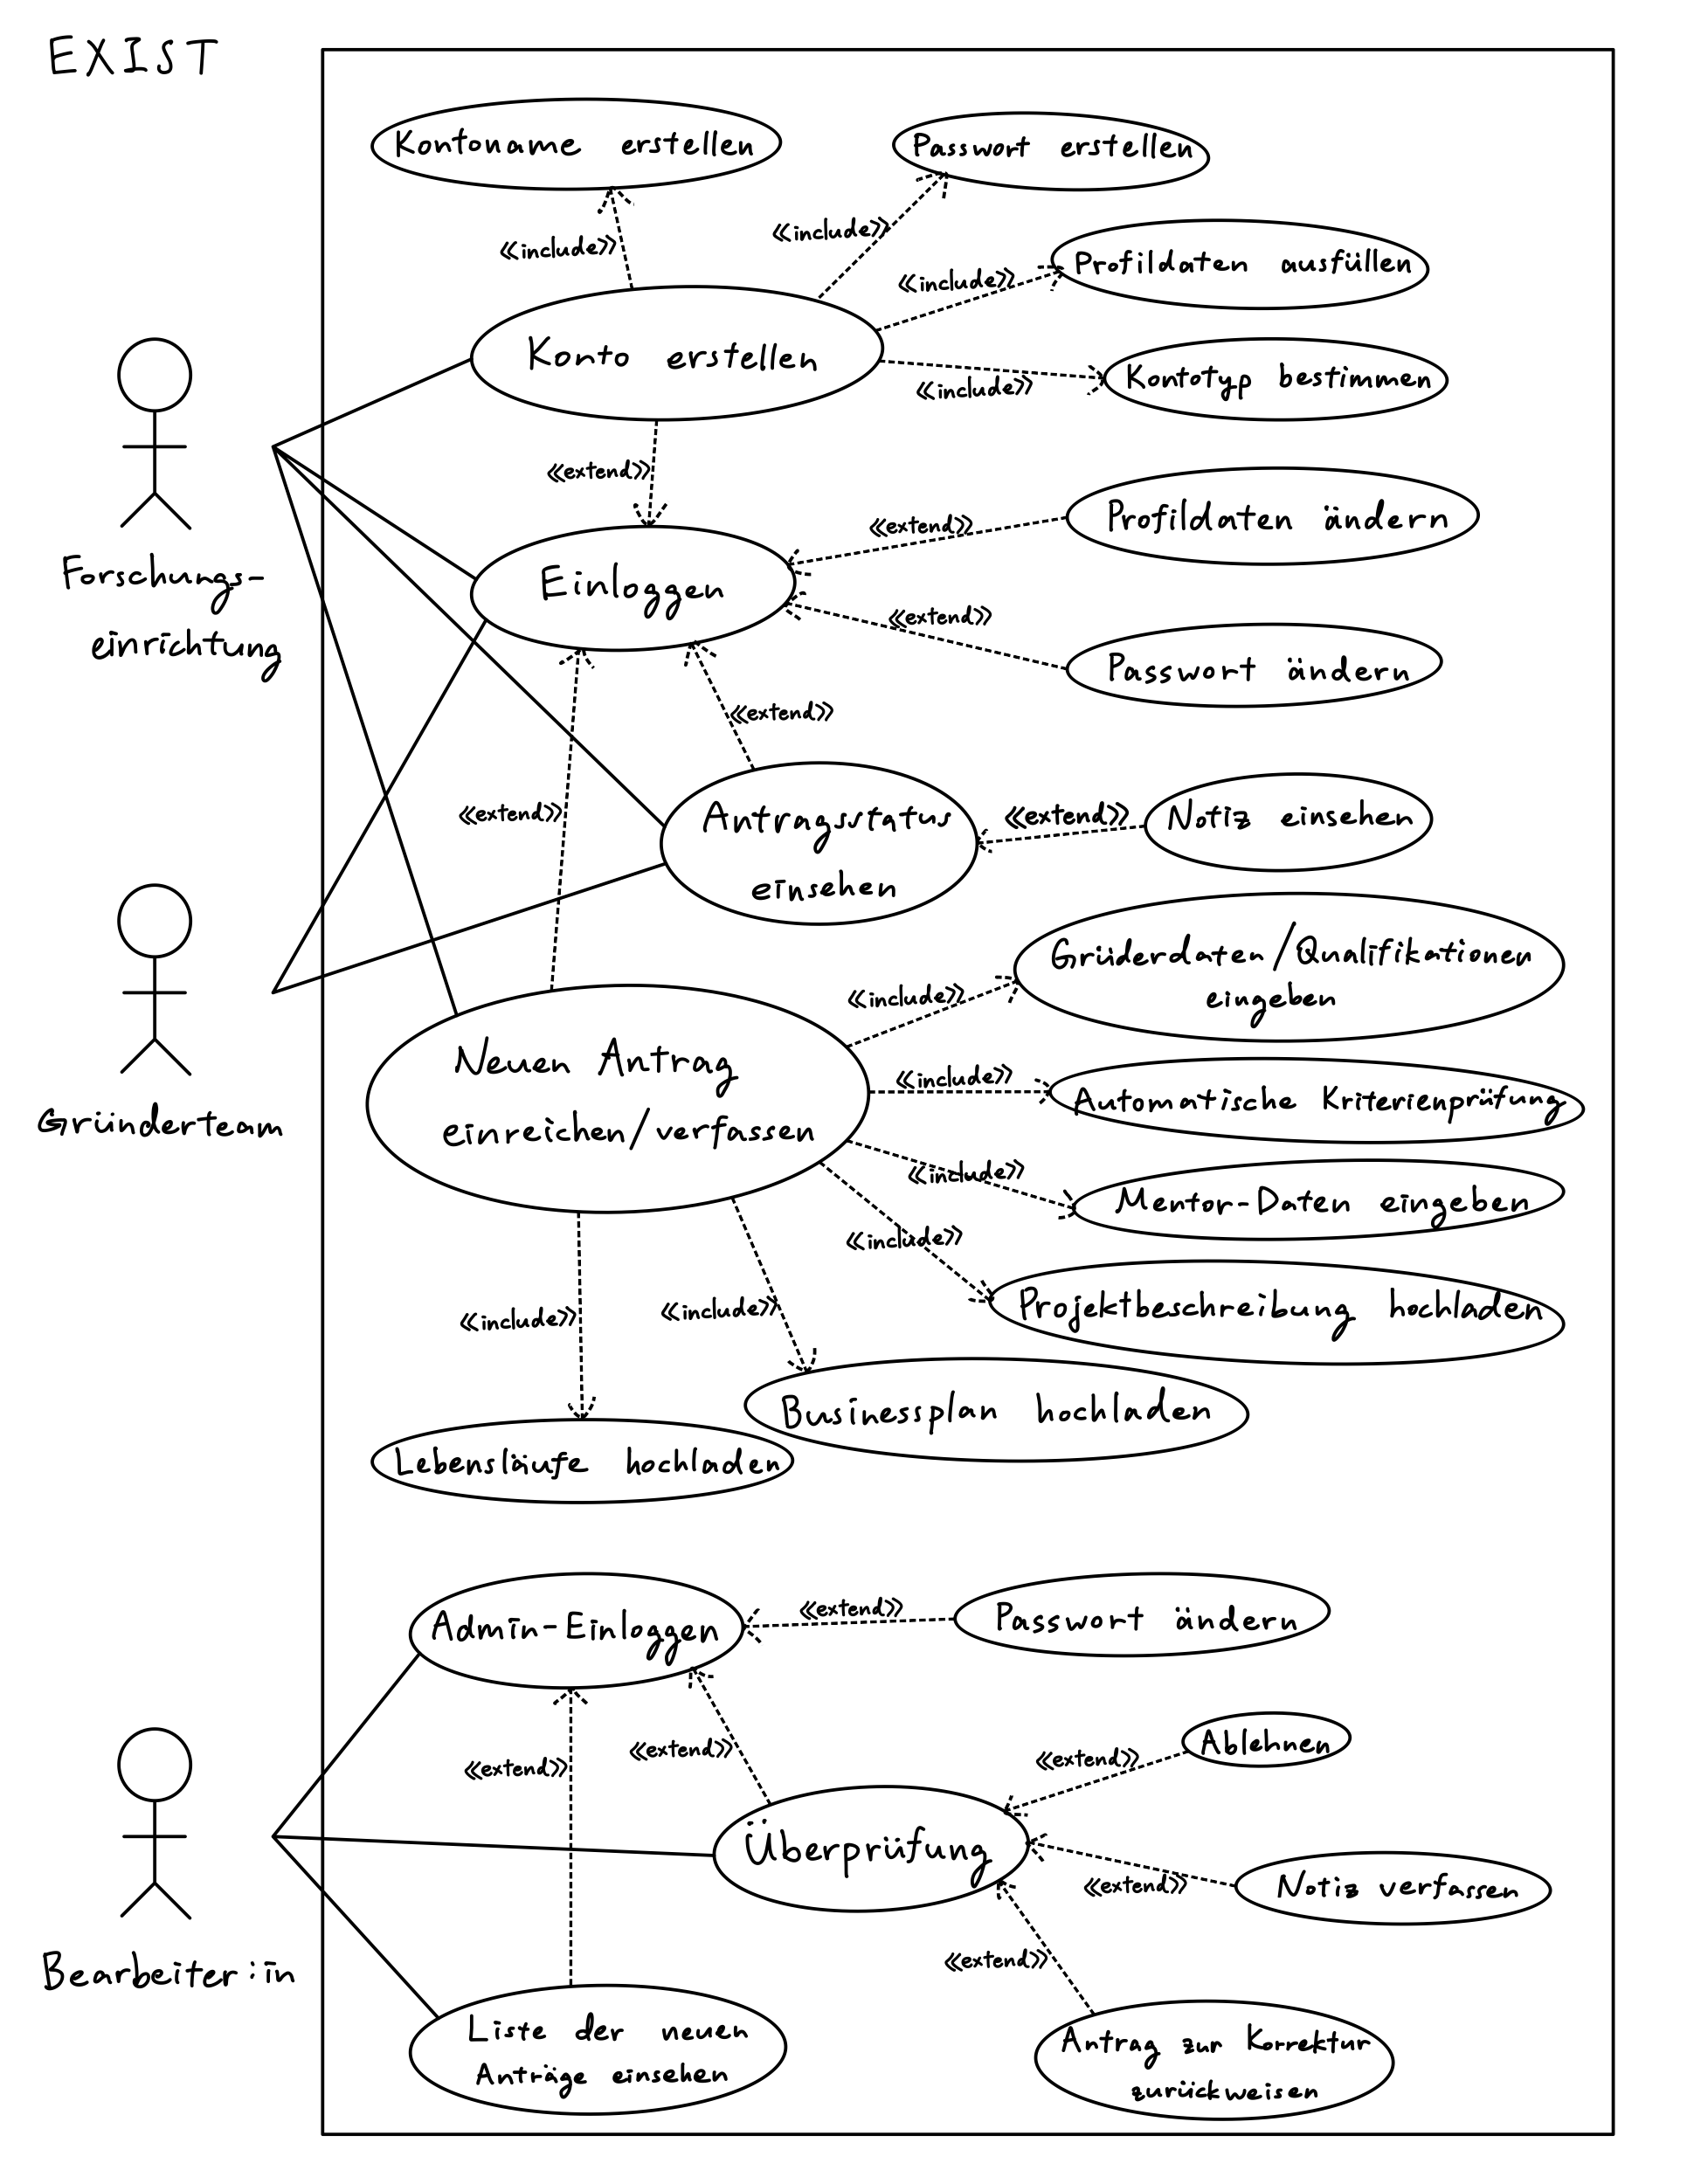
\includegraphics[width=0.8\textwidth]{Use Case Diagramm.png}
\end{center}
\newpage

\subsubsection{Use Case Förderantrag einreichen}
\begin{table}[htbp]
\centering
\begin{tabularx}{\textwidth}{lX}
\midrule
Titel & Förderantrag einreichen\\
Ziel & Antrag für EXIST Förderung erfassen\\
Kurzbeschreibung & Die Forschungseinrichtung füllt das Formular aus\\
Akteure & Forschungseinrichtung\\
Auslösendes Ereignis & Die Forschungseinrichtung beantragt eine Förderung für das Gründerteam und benutzt daher das System\\
\textbf{Ablauf} \\
Vorbedingung & Es liegt kein Antrag des gleichen Gründerteams für das ausgewählte Stipendium vor\\
\hspace{0.5cm} 1. System & Zeigt das Antragsformular zum Eintragen der Daten\\
\hspace{0.5cm} 2. Forschungseinrichtung & Eintragen der Daten ins Formular und klickt auf senden\\
\hspace{0.5cm} 3. Forschungseinrichtung & 3.1 Antrag vollständig und alle Pflichtfelder sind ausgefüllt\\
& 3.2 Antrag nicht vollständig (Alternativ Ablauf 3a)\\
\hspace{0.5cm} 4. System & bestätigt Abgabe der Daten \\
Nachbedingung & Ein Antrag liegt vor\\
\textbf{Alternativer Ablauf}\\
Vorbedingung & Mindestens ein Pflichtfeld ist nicht ausgefüllt oder falsch ausgefüllt\\
\hspace{0.5cm} 3.2a System & Informiert, dass ein Pflichtfeld nicht ausgefüllt oder falsch ausgefüllt ist und aktzeptiert die Abgabe nicht \\
Nachbedingung & Es liegt keine Abgabe vor\\
\bottomrule
\end{tabularx}
\caption{Use Case Förderantrag einreichen}
\end{table}

\newpage

\subsubsection{Use Case Förderantrag überprüfen}
\begin{table}[htbp]
\centering
\begin{tabularx}{\textwidth}{lX}
\midrule
Titel & Förderantrag überprüfen\\
Ziel & Genehmigung oder Ablehnung des Förderantrags\\
Kurzbeschreibung & Bearbeiter:in überprüft das eingereichte Formular und entscheidet über Genehmigung oder Ablehnung\\
Akteure & Bearbeiter:in\\
Auslösendes Ereignis & Ein Förderantrag wurde von einer Forschungseinrichtung eingereicht. Die Bearbeitende Person nutzt das System und entscheidet über den Förderantrag \\
\textbf{Ablauf} \\
Vorbedingung & Ein vollständiger Förderantrag liegt im System vor\\
\hspace{0.5cm} 1. System & zeigt Förderanträge, welche überprüft werden müssen \\
\hspace{0.5cm} 2. Bearbeiter:in & Förderantrag wird überprüft\\
\hspace{0.5cm} 3. Bearbeiter:in & 3.1 Förderantrag wird abgelehnt und "abgelehnt" wird eingetragen\\
& 3.2 Förderantrag wird angenommen und "angenommen" wird eingetragen\\
& 3.3 Es bestehen Unklarheiten und der Status wird nicht verändert (Alternativ Ablauf 3.3a)\\
\hspace{0.5cm} 4. System & bestätigt Eintragung der Entscheidung\\
Nachbedingung & Ein genehmigter oder abgelehnter Förderantrag ist im System eingetragen\\
\textbf{Alternativer Ablauf} \\
Vorbedingung & Antrag nicht eindeutig Entscheidbar\\
\hspace{0.5cm} 3.3a Bearbeiter:in & hinterlässt Notiz für die zuständige Forschungseinrichtung \\
\hspace{0.5cm} 3.3b System & bestätigt Eintragung der Notiz \\
Nachbedingung & Es liegt keine Entscheidung vor und eine Notiz wurde angelegt\\
\bottomrule
\end{tabularx}
\caption{Use Case Förderantrag überprüfen}
\end{table}

\subsubsection{Use Case Information/Status des Förderantrags anzeigen}
\begin{table}[htbp]
\centering
\begin{tabularx}{\textwidth}{lX}
\midrule
Titel & Information/Status eines Förderantrags anzeigen\\
Ziel & Anzeigen des Status und der Daten eines bestehenden Förderantrags\\
Kurzbeschreibung & Die Daten und der Status eines Förderantrags werden dem entsprechenden Akteur angezeigt \\
Akteure & Forschungseinrichtung, Bearbeiter:in, Gründungsteam\\
Auslösendes Ereignis & Förderantrag wurde eingereicht und ein Akteur möchte den Status und die Daten einsehen\\
\textbf{Ablauf} \\
Vorbedingung & Ein vollständiger Förderantrag liegt im System vor\\
\hspace{0.5cm} 1. System & zeigt entsprechenden Förderantrag und den vorliegenden Status an\\
Nachbedingung & Ein vollständiger Förderantrag liegt im System vor\\
\textbf{Alternativer Ablauf} \\
Vorbedingung & \\

Nachbedingung & \\
\bottomrule
\end{tabularx}
\caption{Use Case Information/Status des Förderantrags anzeigen}
\end{table}
\newpage
\subsection{Funktionale Anforderungen}
\begin{table}[htbp]
\centering
\begin{tabularx}{\textwidth}{lX}
\midrule
FA1 & Das System muss Benutzer verwalten können\\
FA2  & Das System muss ein Formular zur Einreichung von Förderanträgen bereitstellen\\
FA3 & Das System muss Förderungsanträge speichern können\\
FA4 & Das System muss Feedback über das erfolgreiche Einreichen des Förderantrags geben\\
FA5 & Das System muss unvollständige oder Fehlerhafte Förderanträge ablehnen\\
FA6 & Das System muss Notizen zu Förderungsanträgen speichern können \\
FA7 & Das System muss den Bearbeitunsgstatus von Förderungsanträgen ändern und speichern können\\
FA8 & Das System muss Daten über Förderungsanträge ausgeben können\\
FA9 & Das System muss Feedback über erfolgreiche Änderungen der Daten geben \\
FA10 & Das System muss Daten löschen lassen können\\

\bottomrule
\end{tabularx}

\caption{Funktionale Anforderungen}
\end{table}
\subsection{Nicht-funktionale Anforderungen}
\begin{table}[htbp]
\centering
\begin{tabularx}{\textwidth}{lX}
\midrule
NFA 1 & Nur Bearbeiter:Innen dürfen Daten ändern können \\
NFA 2 & Forschungseinrichtungen dürfen nur Einblick in selbst eingereichte Förderungsanträge haben\\
NFA 3 & Gründerteams dürfen nur Daten ihres eigenen Antrags sehen\\
NFA 4 & Pflichtfelder müssen eindeutig gekennzeichnet sein \\
NFA 5 & Förderanträge sollen gefiltert werden können \\
\bottomrule
\end{tabularx}
\caption{Nicht Funktionale Anforderungen}
\end{table}


\subsection{Wesentliche Datenobjekte}
\begin{table}[htbp]
\centering
\begin{tabularx}{\textwidth}{lX}
\toprule
Datenobjekt & Beschreibung \\
\midrule
Gründungsteam & Team welches sich mit einer Geschäftsidee für die Gründungsförderung bewirbt\\
Gründer:in & Einzelperson und Teil eines Gründungsteams\\
Bearbeiter:in & Person, die Förderanträge überprüft und über Ablehnung oder Annahme entscheidet\\
Forschungseinrichtung & Antragstellende Einrichtung, welche das Gründungsteam unterstützt\\
Anträge & Dokumente und Informationen zur Beantragung einer Förderung\\
Notiz & Bemerkung der Bearbeiter:in zu einem Antrag \\
Gründungsidee & Innovative Idee zur Unternehmensgründung eines Gründungsteams \\
Mentor:in & Berät und unterstützt Gründungsteams bei fachlichen Fragen \\
Businessplan & Dokument zur Beschreibung eines Geschäftsmodells, der Strategie und wirtschaftlicher Planung\\
Ansprechpartner:in & Verantwortliche Kontaktperson der Forschungseinrichtung\\
Lebenslauf & Dokument mit Lebenslauf einer Gründer:in\\
\bottomrule
\end{tabularx}
\caption{Wesentliche Datenobjekte}
\end{table}
\newpage


\section{Konzeptueller Entwurf}
\begin{center}
    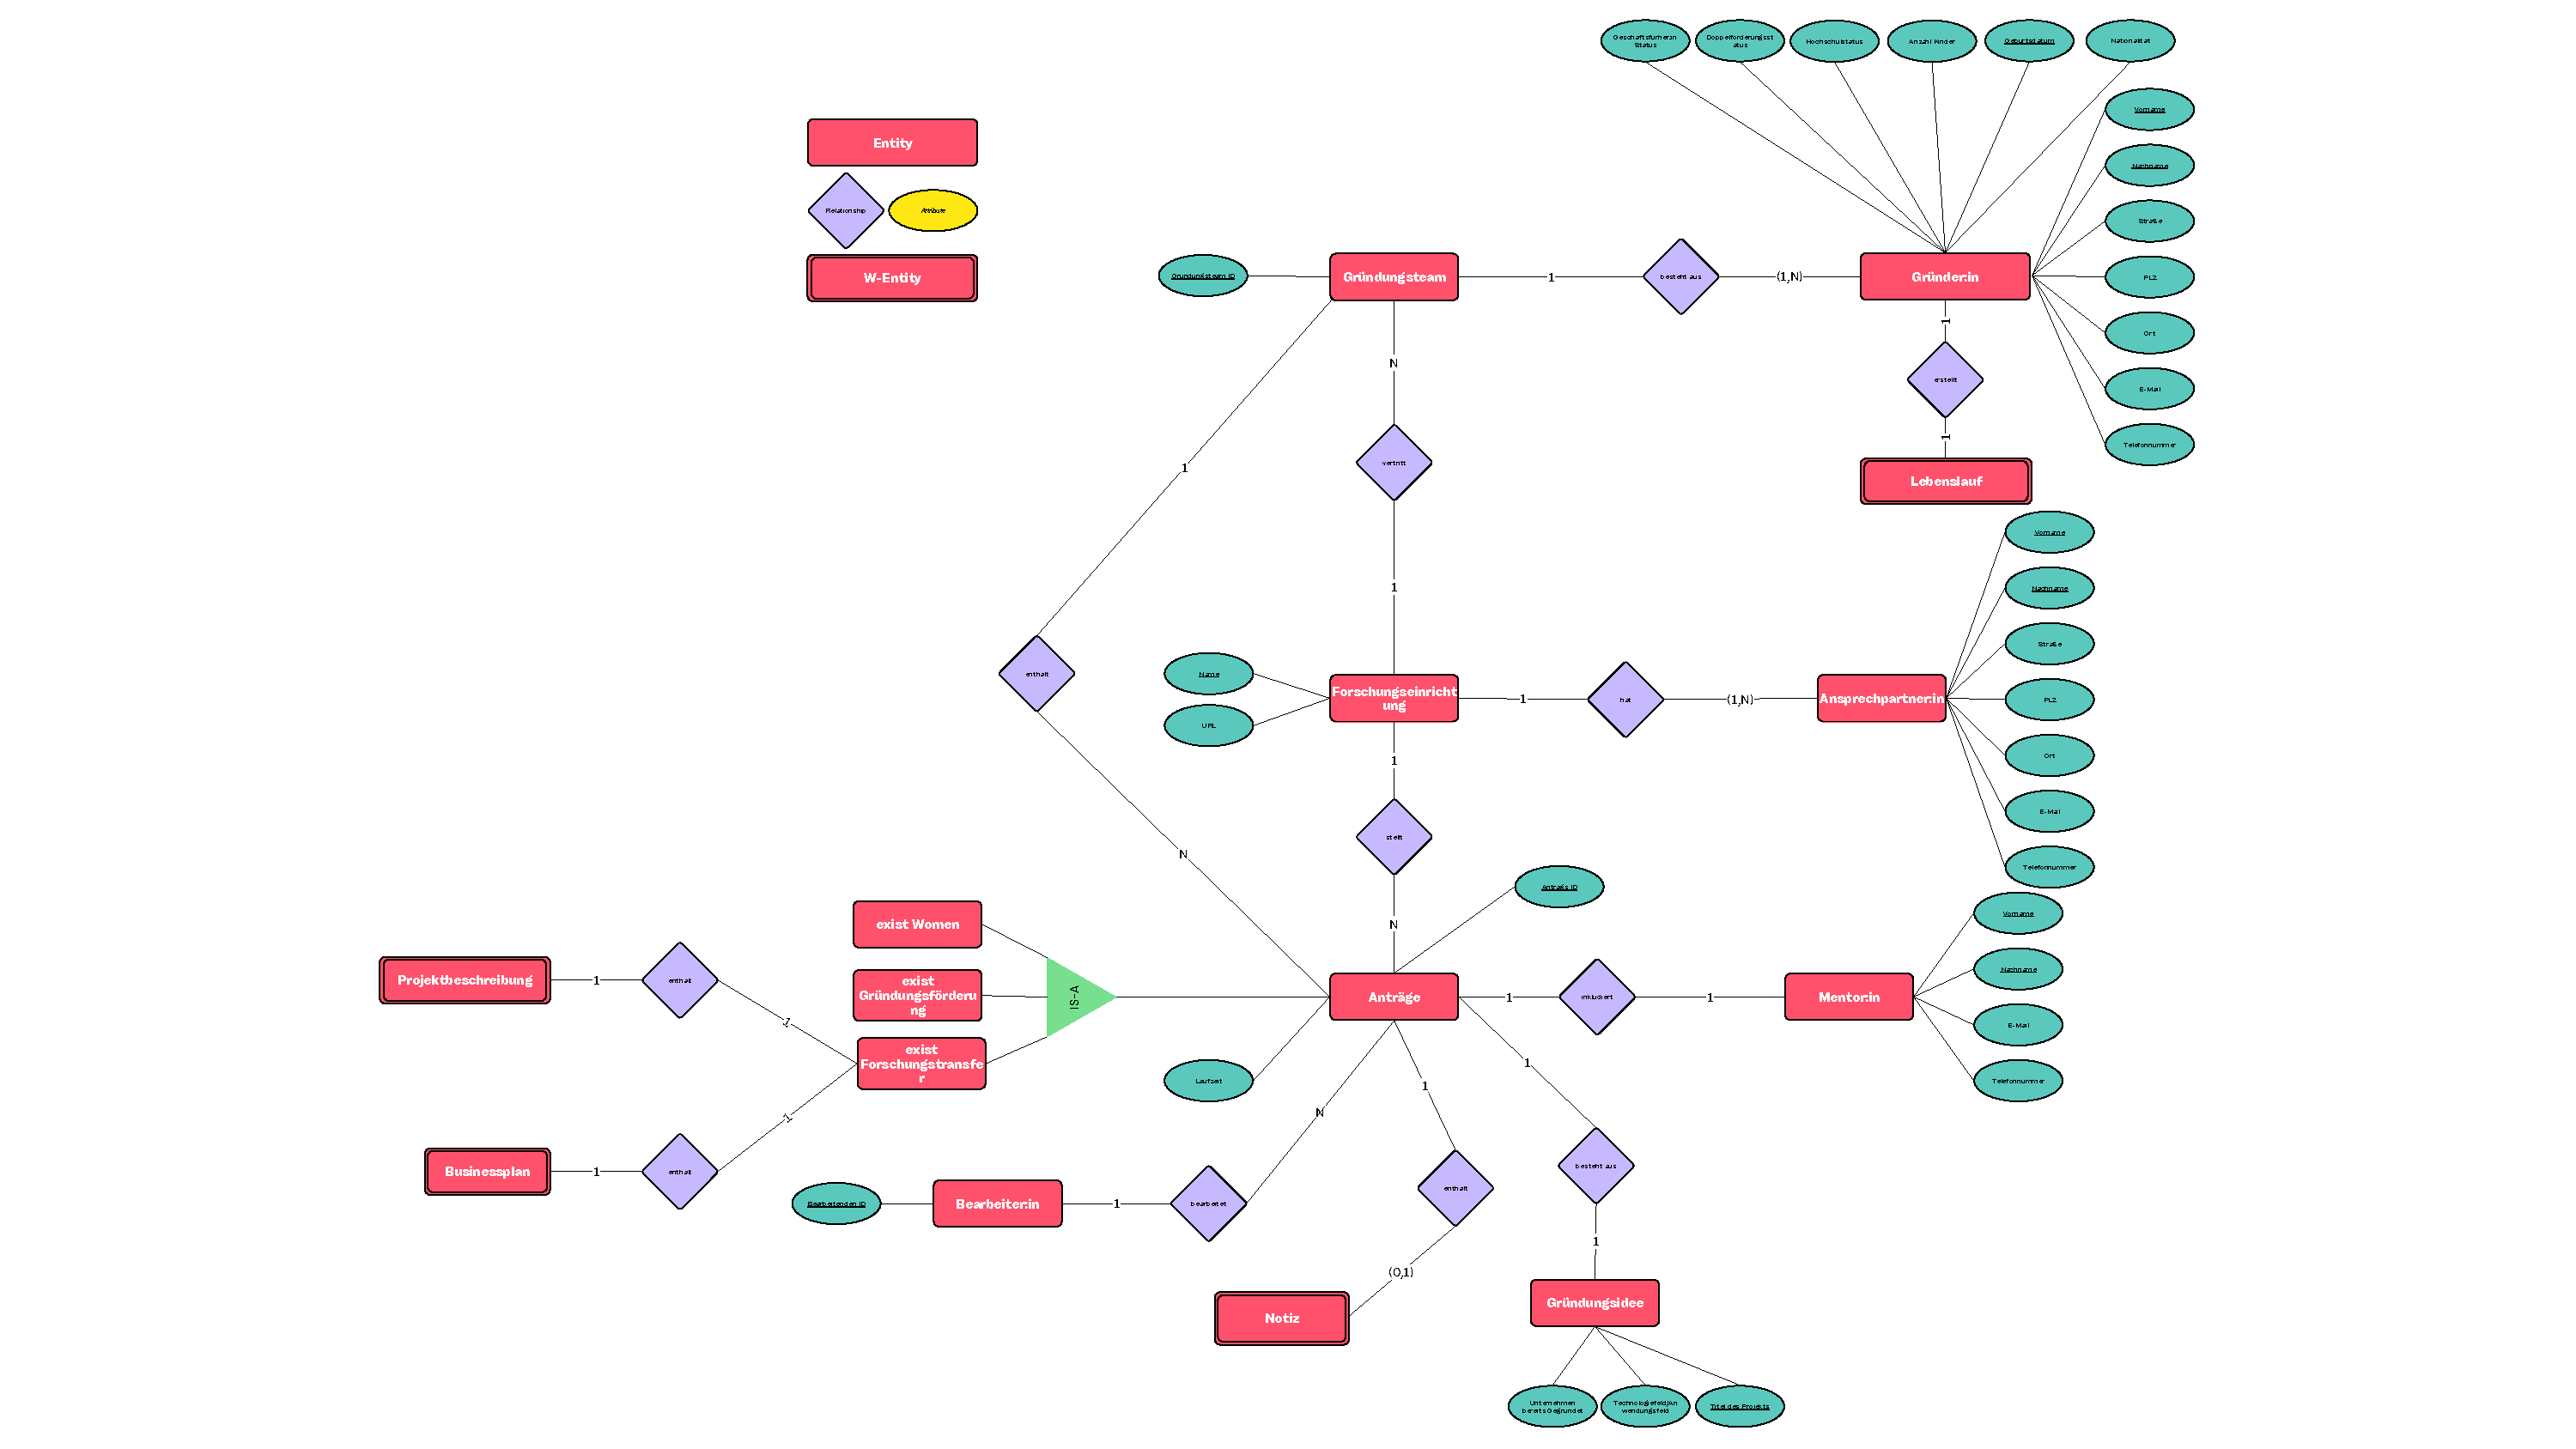
\includegraphics[
        width=1.2\textwidth,
        height=0.8\textheight,
        trim=7cm 0cm 2cm 0cm,
        clip
    ]{ERdiagramm.pdf}
\end{center}
\newpage


\section{Logischer Entwurf}

Der logische Entwurf überführt das konzeptuelle ER-Modell in das relationale Datenmodell. Im Folgenden ist das aktualisierte Schema basierend auf unserer Datenbank-Implementierung dargestellt. Primärschlüssel sind unterstrichen.

\textbf{PLZ/Ort} (\underline{PLZ}, Ort)

\textbf{Forschungseinrichtung} (\underline{Einrichtung ID}, Name, URL)

\textbf{Ansprechpartner:in} (\underline{Ansprechpartner ID}, Vorname, Nachname, Straße, PLZ, E-Mail, Telefon, Einrichtung ID)\\
Fremdschlüssel (Einrichtung ID, PLZ)

\textbf{Mentor:in} (\underline{Mentor ID}, Vorname, Nachname, E-Mail, Telefon)

\textbf{Bearbeiter:in} (\underline{Bearbeiter ID}, Vorname, Nachname, E-Mail)

\textbf{Gründungsteam} (\underline{Team ID}, Team Name, Einrichtung ID)\\
Fremdschlüssel (Einrichtung ID)

\textbf{Gründer:in} (\underline{Gründer ID}, Vorname, Nachname, Geburtsdatum, Straße, PLZ, E-Mail, Telefon, Nationalität, Anzahl Kinder, Hochschulstatus, Team ID)\\
Fremdschlüssel (PLZ, Team ID)

\textbf{Benutzer} (\underline{Benutzer ID}, E-Mail, Passwort, Rolle, Ansprechpartner ID, Gründer ID, Bearbeiter ID, Erstellt am, Letzter Login, Ist aktiv)\\
Fremdschlüssel (Ansprechpartner ID, Gründer ID, Bearbeiter ID)

\textbf{Dokumente} (\underline{Dokument ID}, Dateiname, Dateityp, Datei, Hochgeladen am)

\textbf{Lebenslauf} (\underline{Gründer ID}, Dokument ID)\\
Fremdschlüssel (Gründer ID, Dokument ID)

\textbf{Antrag} (\underline{Antrag ID}, Gründungstitel, Status, Programm, Einreichungsdatum, Zuletzt aktualisiert, Mentor ID, Team ID, Bearbeiter ID, Einrichtung ID)\\
Fremdschlüssel (Einrichtung ID, Mentor ID, Team ID, Bearbeiter ID)

\textbf{Gründungsidee} (\underline{Antrag ID}, Titel, Bereich, Unternehmen)\\
Fremdschlüssel (Antrag ID)

\textbf{Notiz} (\underline{Antrag ID}, \underline{Zeitstempel}, Inhalt, Dokument ID)\\
Fremdschlüssel (Antrag ID, Dokument ID)

\textbf{Antrag Status Historie} (\underline{Historie ID}, Antrag ID, Bearbeiter ID, Alter Status, Neuer Status, Änderungsdatum)\\
Fremdschlüssel (Antrag ID, Bearbeiter ID)

\textbf{exist Women} (\underline{Antrag ID}, Motivationspapier ID)\\
Fremdschlüssel (Antrag ID, Motivationspapier ID)

\textbf{exist Gründungsförderung} (\underline{Antrag ID}, Ideenpapier ID)\\
Fremdschlüssel (Antrag ID, Ideenpapier ID)

\textbf{exist Forschungstransfer} (\underline{Antrag ID}, Projektbeschreibung ID, Businessplan ID)\\
Fremdschlüssel (Antrag ID, Projektbeschreibung ID, Businessplan ID)

\subsection{Normalisierung}
Das vorliegende Datenbankschema befindet sich in der \textbf{3. Normalform (3NF)}. 

Alle Attribute sind atomar gespeichert (z.B. die Aufteilung in \texttt{Straße} und \texttt{PLZ}). Durch die durchgehende Verwendung von künstlichen Primärschlüsseln (Surrogate Keys wie \texttt{Antrag ID} oder \texttt{Gründer ID}) sind alle Nicht-Schlüssel-Attribute voll funktional vom jeweiligen Primärschlüssel abhängig. Transitive Abhängigkeiten wurden durch die Auslagerung in separate Tabellen konsequent aufgelöst. Ein Beispiel hierfür ist die Auslagerung des Ortsnamens in die Tabelle \textbf{PLZ/Ort}, wodurch Redundanzen in den Tabellen \textbf{Gründer:in} und \textbf{Ansprechpartner:in} vermieden werden.


\newpage
\section{Datendefinition}
Die Umsetzung des logischen Entwurfs in die physische Datenbankstruktur erfolgte mittels SQL Data Definition Language (DDL). Für alle Relationen wurden entsprechende Tabellen in einer MySQL-Datenbank angelegt. Dabei wurden die Datentypen passend gewählt (z.B. \texttt{ENUM} für Statuswerte, \texttt{LONGBLOB} für PDF-Dokumente) und alle Primär- und Fremdschlüssel-Constraints (inklusive \texttt{ON DELETE CASCADE} / \texttt{ON DELETE SET NULL} wo sinnvoll) implementiert.

Zusätzlich wurde, wie in den Anforderungen gefordert, eine Sicht (View) erstellt:
\begin{itemize}
    \item \textbf{\texttt{view\_antrag\_uebersicht}}: Dieser View verknüpft die Tabelle \texttt{antrag} mit der \texttt{forschungseinrichtung} und liefert eine kompakte Übersicht der Antragsdaten (Antrag ID, Titel, Programm, Status, Einreichungsdatum, Name der Einrichtung). Er dient der vereinfachten Datenabfrage für das Dashboard.
\end{itemize}

\section{Physischer Entwurf}
Um die Performance der SQL-Anfragen im Dashboard zu optimieren, wurden im physischen Entwurf spezifische Indizes (B-Trees in MySQL) angelegt. Gemäß den Projektanforderungen wurden mindestens zwei Indizes definiert:
\begin{itemize}
    \item \textbf{\texttt{idx\_antrag\_status} auf \texttt{antrag(status)}}: Da im Dashboard häufig Anträge nach ihrem Bearbeitungsstatus (z.B. "eingereicht", "in\_pruefung") gefiltert und gruppiert werden, beschleunigt dieser Index die entsprechenden Such- und Aggregationsanfragen erheblich.
    \item \textbf{\texttt{idx\_gruender\_nachname} auf \texttt{gruender(nachname)}}: Dieser Index optimiert die Suche nach bestimmten Gründer:innen innerhalb des Systems.
\end{itemize}

\section{Implementierung des Tools (Dashboard)}
Als Frontend-Schnittstelle zur Datenbank wurde ein interaktives Tool in Form eines Web-Dashboards implementiert. 
\begin{itemize}
    \item \textbf{Technologie-Stack}: Das Tool wurde in \textbf{Python} unter Verwendung des Frameworks \textbf{Streamlit} entwickelt. Die Anbindung an die MySQL-Datenbank erfolgt über die Bibliothek \texttt{mysql-connector-python}.
    \item \textbf{Funktionalität}: Das Dashboard setzt die rollenbasierte Zugriffskontrolle (RBAC) aus der Anforderungsanalyse um. Nach dem Login (als Ansprechpartner:in, Gründer:in oder Bearbeiter:in) präsentiert das System maßgeschneiderte Ansichten. Es ermöglicht das Ausfüllen von Antragsformularen, den Upload von PDF-Dokumenten (gespeichert als BLOBs in der Datenbank), die Statusänderung von Anträgen sowie die Generierung von statistischen Auswertungen (z.B. Balkendiagramme der Anträge pro Programm).
    \item \textbf{Transaktionssicherheit}: Komplexe Datenbankoperationen, wie das Einreichen eines Antrags (welches Inserts in die Haupttabelle \texttt{antrag} sowie die programmspezifischen Tabellen wie \texttt{exist\_women} erfordert), werden in Transaktionen (\texttt{connection.commit()} / \texttt{connection.rollback()}) gekapselt, um die Datenkonsistenz stets zu gewährleisten.
\end{itemize}


\newpage
\section{Datenbankanfragen (SQL Queries)}
Für die Implementierung unseres Dashboards in Python/Streamlit haben wir verschiedene SQL-Anfragen definiert. Im Folgenden sind 10 essenzielle Anfragen aufgelistet, welche die gestellten Anforderungen (Aggregation, Join, Sub-Anfrage, parametrisierte Queries) erfüllen. In der Python-Implementierung werden die Variablen als Parameter (z.B. \texttt{\%s}) übergeben, um SQL-Injection zu verhindern.

\textbf{1. Aggregation \& Gruppierung (Dashboard-Statistik für Bearbeiter)}\\
Diese Abfrage ermittelt die Anzahl der Anträge pro Förderprogramm und Status.
\begin{minted}{sql}
SELECT programm, status, COUNT(*) AS anzahl_antraege
FROM antrag
GROUP BY programm, status
ORDER BY programm, status;
\end{minted}

\textbf{2. Sub-Anfrage (Dokumentenabruf für EXIST-Women)}\\
Diese Abfrage nutzt eine Sub-Query, um das Motivationspapier für einen spezifischen Antrag abzurufen.
\begin{minted}{sql}
SELECT * FROM dokumente 
WHERE dokument_id = (
    SELECT motivationspapier_id 
    FROM exist_women 
    WHERE antrag_id = %s
);
\end{minted}

\textbf{3. JOIN-Abfrage (Antragsübersicht für Gründer)}\\
Diese Anfrage verknüpft Anträge mit den zugehörigen Gründern, um nur die Anträge des eigenen Teams anzuzeigen.
\begin{minted}{sql}
SELECT a.antrag_id, a.gruendungstitel, a.programm, a.status, a.einreichungsdatum
FROM antrag a
JOIN gruender g ON a.team_id = g.team_id
WHERE g.gruender_id = %s
ORDER BY a.einreichungsdatum DESC;
\end{minted}

\textbf{4. Mehrfach-JOIN (Detaillierte Antragsdaten)}\\
Diese Abfrage holt alle relevanten Stammdaten zu einem spezifischen Antrag.
\begin{minted}{sql}
SELECT a.*, t.*, f.*
FROM antrag a
LEFT JOIN gruendungsteam t ON a.team_id = t.team_id
LEFT JOIN forschungseinrichtung f ON a.einrichtung_id = f.einrichtung_id
WHERE a.antrag_id = %s;
\end{minted}

\textbf{5. UNION (Dokumentenabruf für Forschungstransfer)}\\
Für den Forschungstransfer müssen Projektbeschreibung und Businessplan abgerufen werden.
\begin{minted}{sql}
SELECT * FROM dokumente 
WHERE dokument_id IN (
    SELECT projektbeschreibung_id FROM exist_forschungstransfer WHERE antrag_id = %s
    UNION
    SELECT businessplan_id FROM exist_forschungstransfer WHERE antrag_id = %s
);
\end{minted}

\textbf{6. Parametrisierter INSERT (Gründer registrieren)}\\
Sicheres Einfügen neuer Nutzerdaten über das Streamlit-Formular.
\begin{minted}{sql}
INSERT INTO gruender (
    vorname, nachname, geburtsdatum, strasse, plz, 
    email, telefon, nationalitaet, anzahl_kinder, hochschulstatus
) VALUES (%s, %s, %s, %s, %s, %s, %s, %s, %s, %s);
\end{minted}

\textbf{7. UPDATE (Statusänderung durch Bearbeiter)}\\
\begin{minted}{sql}
UPDATE antrag
SET status = %s
WHERE antrag_id = %s;
\end{minted}

\textbf{8. UPSERT / ON DUPLICATE KEY UPDATE (Lebenslauf speichern)}\\
Diese Abfrage stellt sicher, dass pro Gründer nur ein aktueller Lebenslauf referenziert wird.
\begin{minted}{sql}
INSERT INTO lebenslauf (gruender_id, dokument_id)
VALUES (%s, %s) 
ON DUPLICATE KEY UPDATE dokument_id = VALUES(dokument_id);
\end{minted}

\textbf{9. Login \& Authentifizierung}\\
\begin{minted}{sql}
SELECT benutzer_id, email, passwort, rolle, 
       ansprechpartner_id, gruender_id, bearbeiter_id
FROM benutzer
WHERE email = %s AND passwort = %s;
\end{minted}

\textbf{10. Datenauswahl für Dropdown-Menüs (PLZ \& Ort)}\\
\begin{minted}{sql}
SELECT plz, ort FROM plz_ort;
\end{minted}



\end{document}


